% \begin{frame}{A Theory of Onset Temperature in 2D: Young's Modulus as $T \to T_\mathrm{KT}$}

% \begin{columns}

% \begin{column}[T]{0.45\textwidth}

% \begin{itemize}
%     \item<2->Pick an intermediate time $\Delta t \ll \tau_\mathrm{eq}$ and measure strain fluctuations at $t = \Delta t$
%     \only<2-3> 
%     {
%     \begin{equation*}
%     \frac{1}{Y^\mathrm{R}} = \beta A_0 \left(\left\langle\hat{\epsilon}_{i j} \hat{\epsilon}_{i j}\right\rangle+\frac{1}{2}\left\langle\hat{\epsilon}_{i i}\hat{\epsilon}_{k k}\right\rangle\right)
%     \end{equation*}
%     }
%     \begin{figure}
%     \begin{overprint}
%     \onslide<4-17>\centering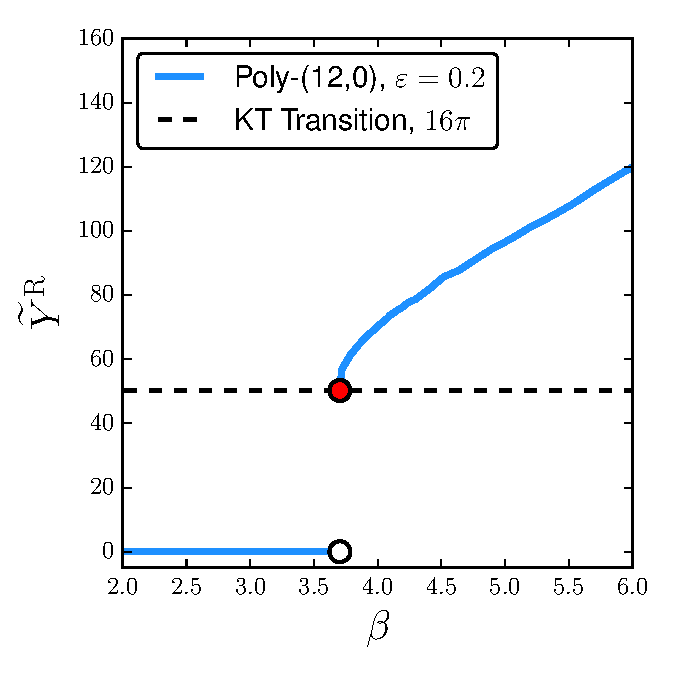
\includegraphics[height=0.65\textheight]{9.d-kt_keim/Yrenorm_poly12.pdf}\caption{The predicted Young's modulus according to RG calculations (discontinuity at $T=T_\mathrm{KT}$)}
    
%     \onslide<18->\centering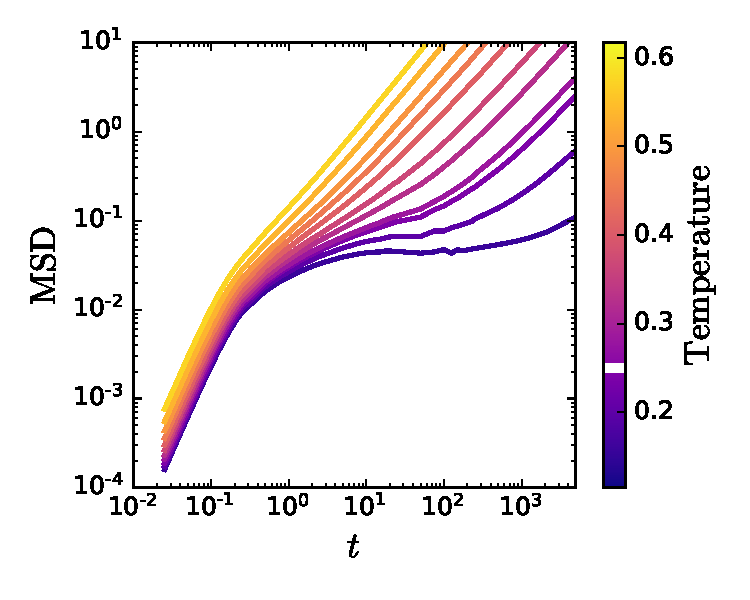
\includegraphics[height=0.625\textheight]{9.d-kt_keim/msd_poly12.pdf}\caption{MSD Data of Poly-(12,0) around the onset temperature, which is qualitatively similar to experimental data.}
%     \end{overprint}
%     \end{figure}
    
% \end{itemize}

% \end{column}

% \begin{column}[T]{0.5\textwidth}

% \begin{itemize}
%     \item<5-> Similar measurements have been done in an \textit{experimental} study (Klix, Maret, and Keim \textit{Phys. Rev. X} 2015)
%     \begin{figure}
%     \begin{overprint}
%     \onslide<6>\centering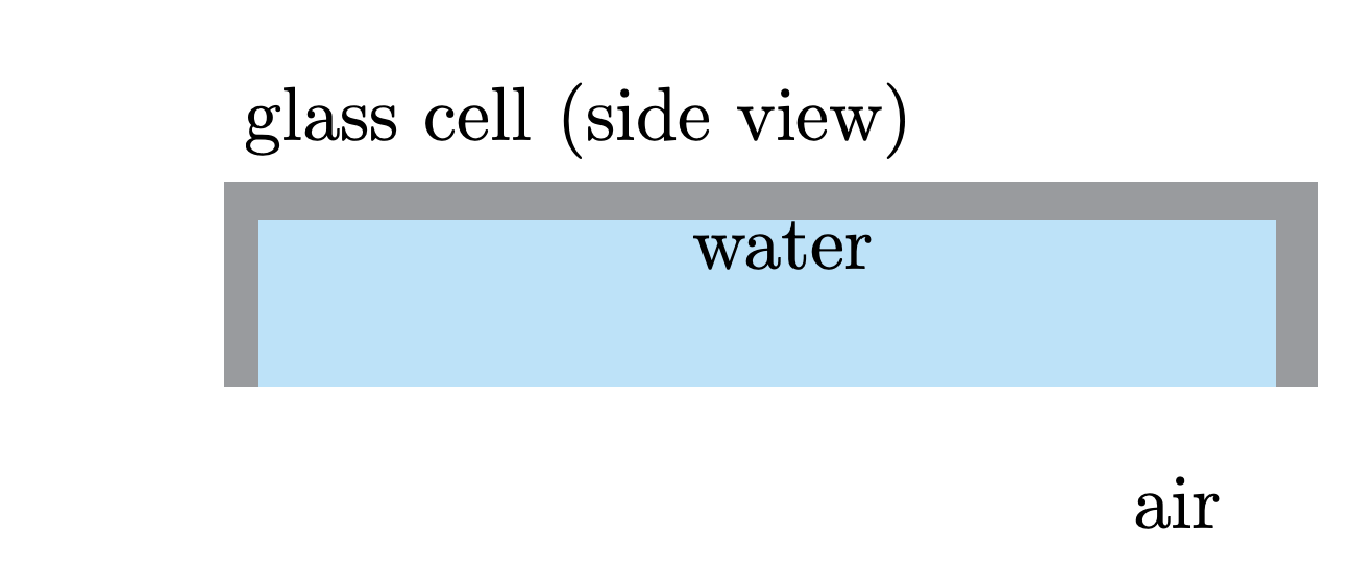
\includegraphics[width=\linewidth]{9.d-kt_keim/keim_setup_0.pdf}\caption{A colloidal system (polystyrene spheres) confined to a flat water-air interface (Ebert, et.al. \textit{Rev. Sci. Instrum} 2009).}
%     \onslide<7>\centering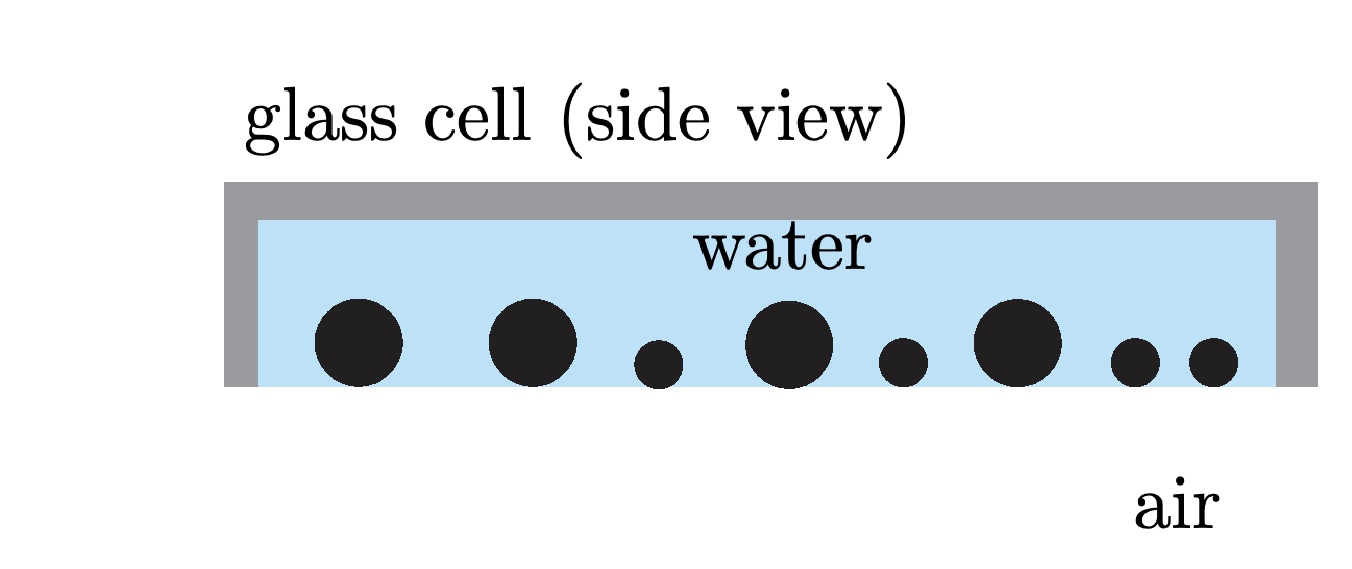
\includegraphics[width=\linewidth]{9.d-kt_keim/keim_setup_1.pdf}\caption{A colloidal system (polystyrene spheres) confined to a flat water-air interface (Ebert, et.al. \textit{Rev. Sci. Instrum} 2009).}
%     \onslide<8>\centering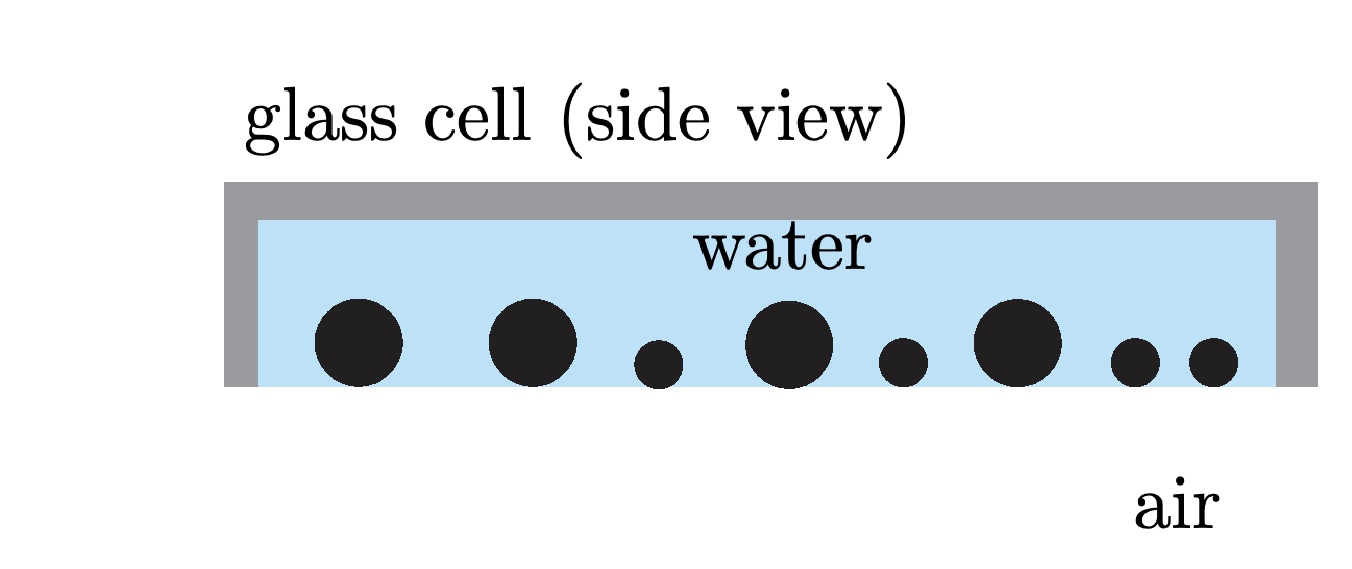
\includegraphics[width=\linewidth]{9.d-kt_keim/keim_setup_1.pdf}\caption{Each sphere is doped with magnetite}
%     \onslide<9-10>\centering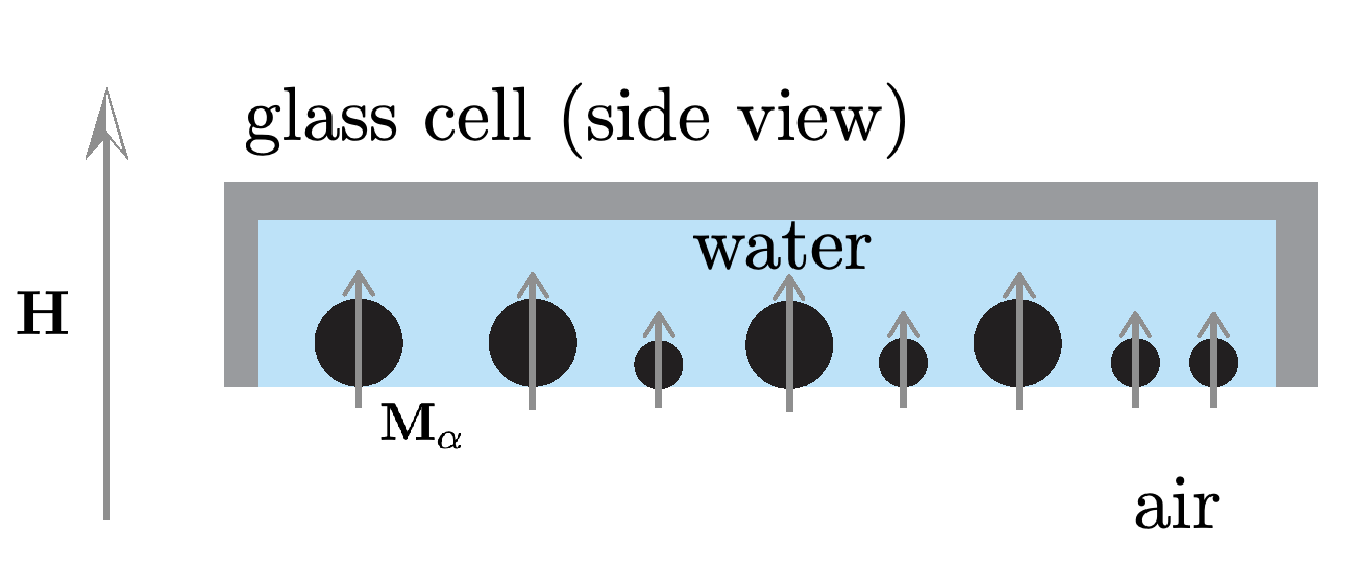
\includegraphics[width=\linewidth]{9.d-kt_keim/keim_setup_2.pdf}\caption{Each sphere is doped with magnetite $\to$ tuning of pair dipolar interaction between particles}\onslide<10>{$$\km{ \text{Coupling strength} \ \Gamma} \sim \beta H^2 $$}
%     \onslide<11>\centering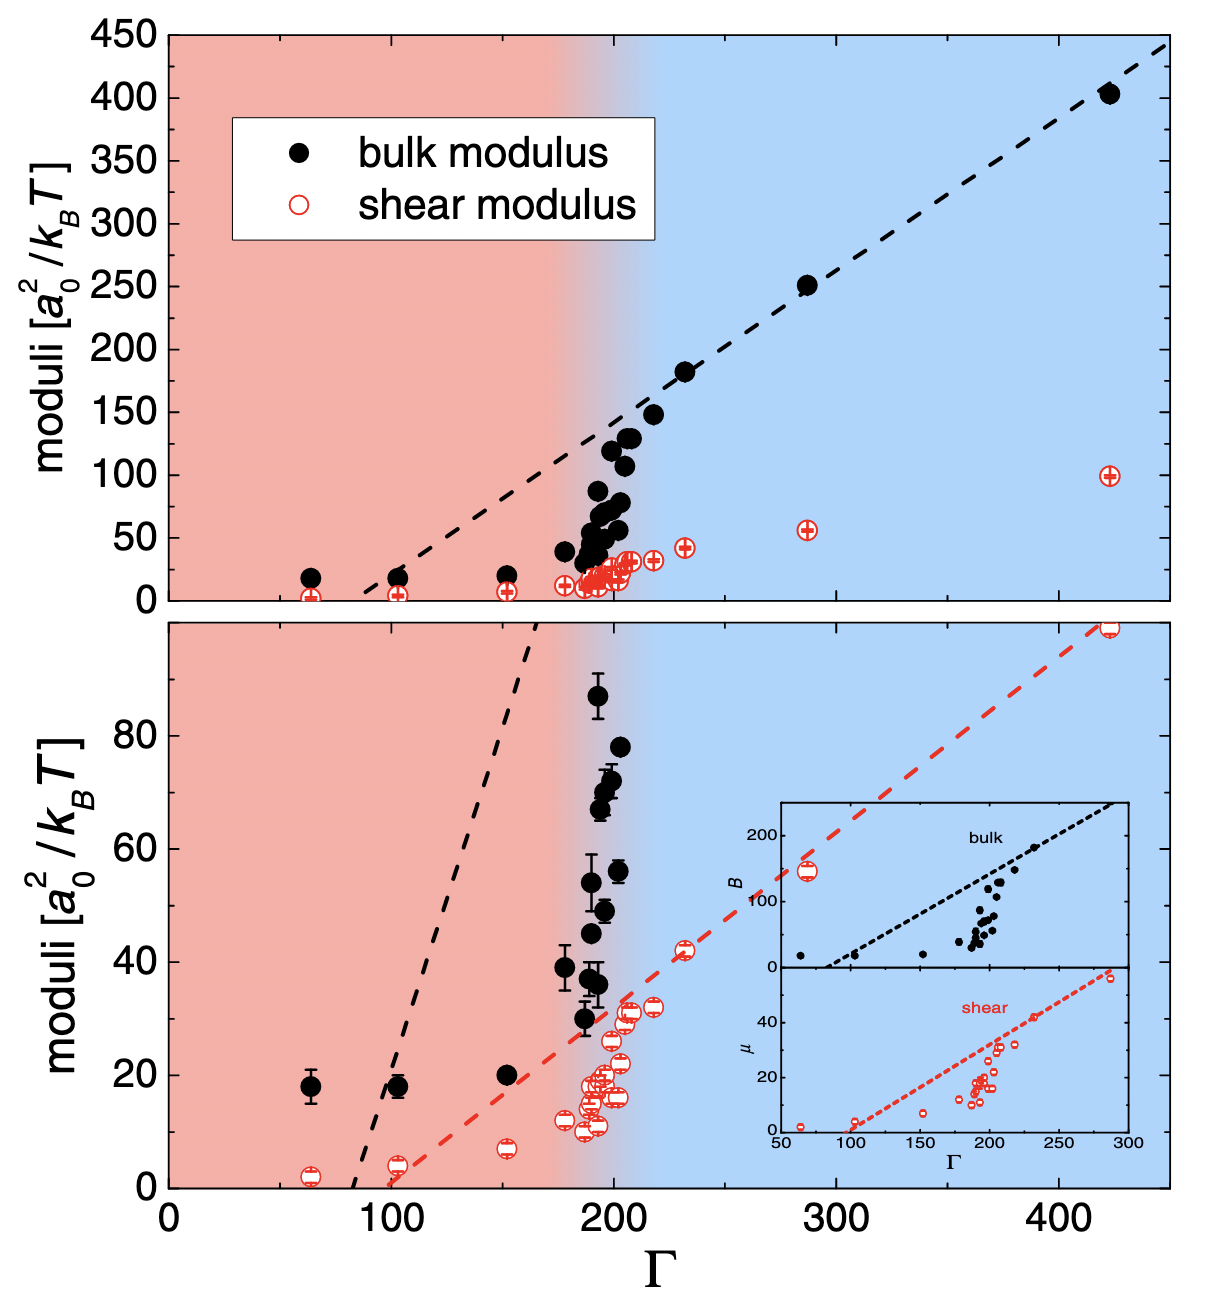
\includegraphics[height=0.6\textheight]{9.d-kt_keim/keim_screenshot.png}\caption{Bulk and shear moduli data at different $\Gamma$ values  (Klix, Maret, and Keim \textit{Phys. Rev. X} 2015).}
%     \onslide<12>\raggedright\vspace{15pt}{\textit{Concerning the height of the jumps, we are not aware of predictions of universal behavior of elasticity in thermal amorphous systems as, e.g., the famous $16 \pi \approx 50.26$ for Young's modulus in $2 \mathrm{D}$ melting [40], but the measured values in glass and crystal are of} \textbf{the same order.} 
%     \vspace{5pt}
    
%     \hfill ---- Klix, Maret, and Keim \textit{Phys. Rev. X} 2015}
%     \onslide<13>\centering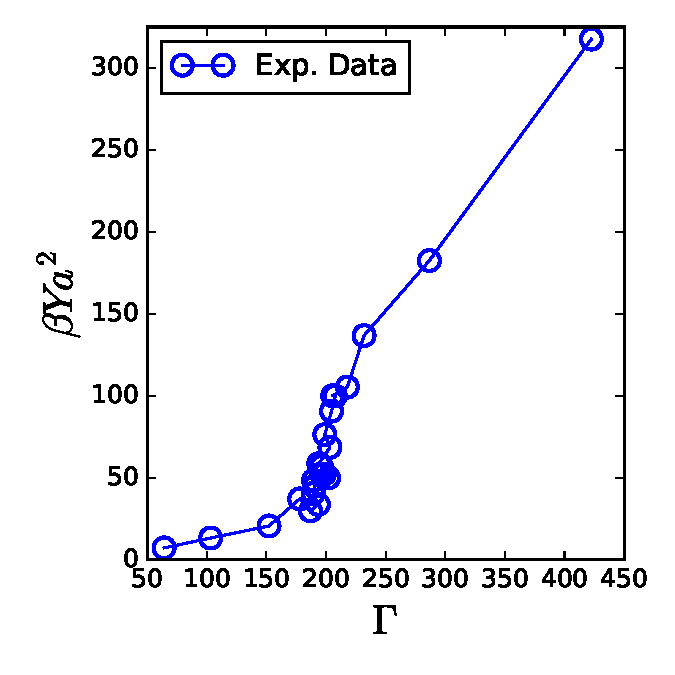
\includegraphics[height=0.6\textheight]{9.d-kt_keim/youngmodulus_keim_0.pdf}\caption{Young's modulus data, (re)computed from the bulk/shear moduli data.}
%     \onslide<14>\centering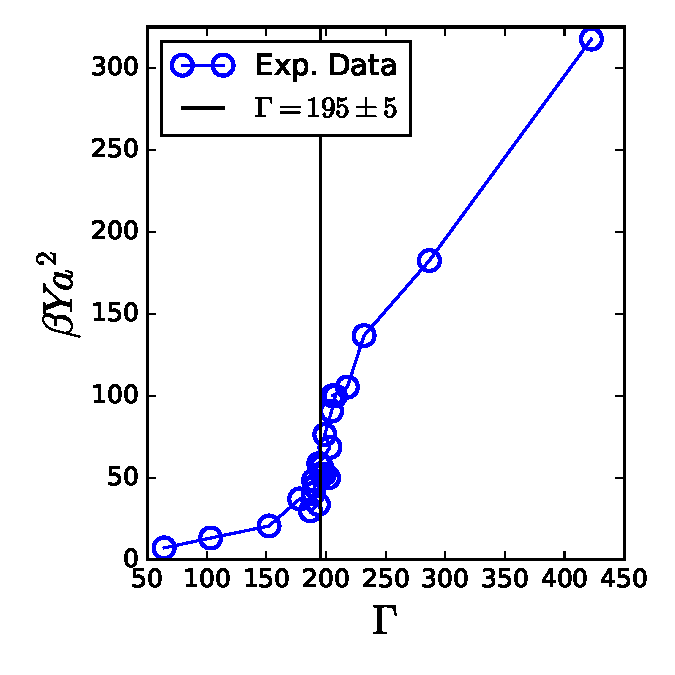
\includegraphics[height=0.6\textheight]{9.d-kt_keim/youngmodulus_keim_1.pdf}\caption{Young's modulus data, (re)computed from the bulk/shear moduli data.}
%     \onslide<15>\centering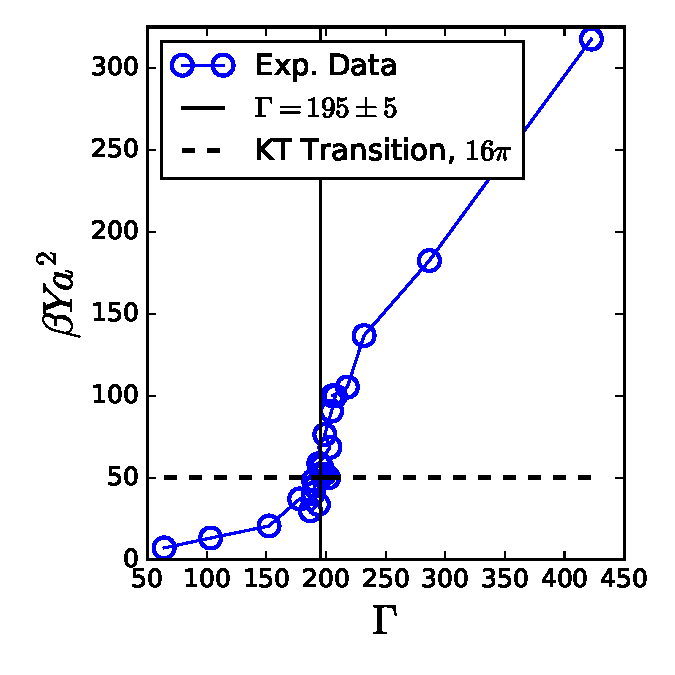
\includegraphics[height=0.6\textheight]{9.d-kt_keim/youngmodulus_keim_2.pdf}\caption{Young's modulus data, (re)computed from the bulk/shear moduli data.}
%     \onslide<16>\centering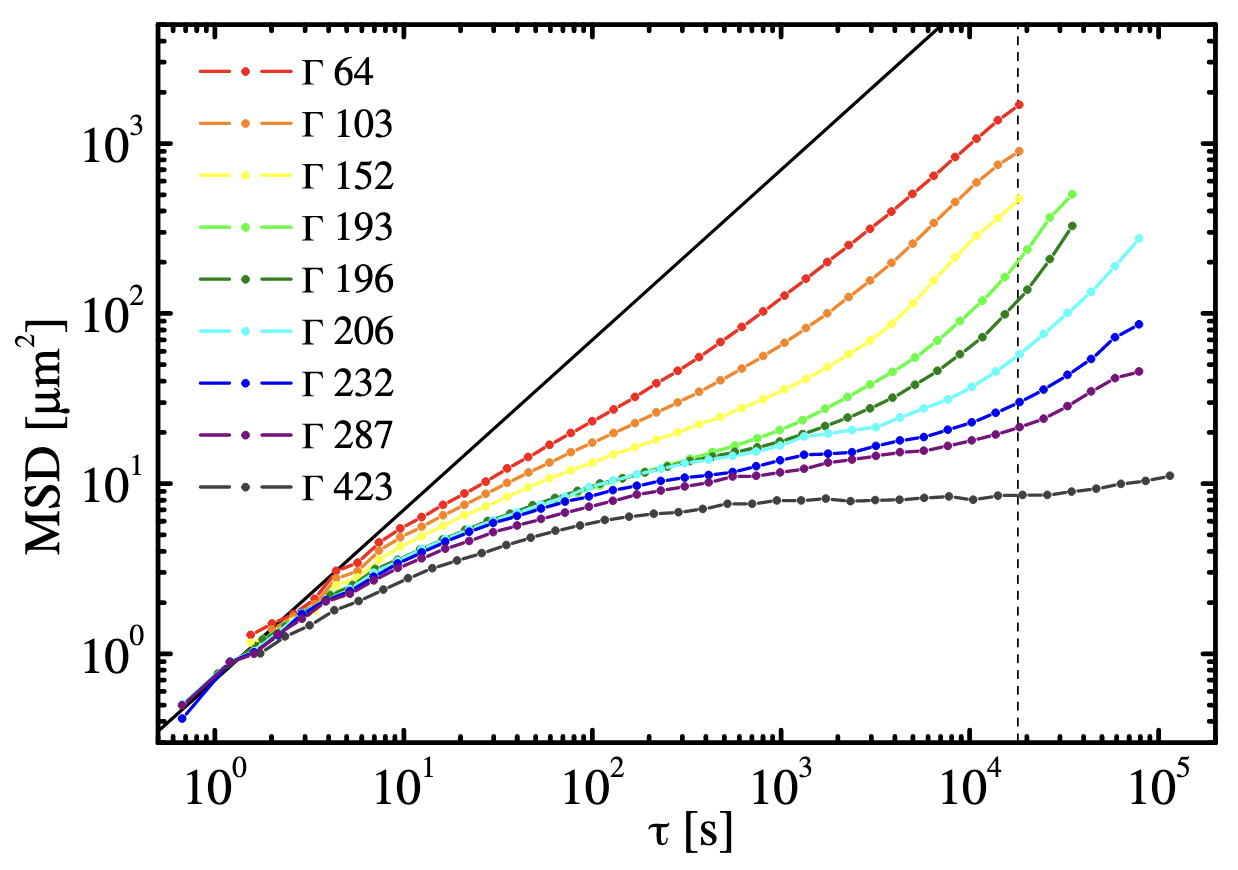
\includegraphics[width=0.9\linewidth]{9.d-kt_keim/msd_keim.png}\caption{Their MSD data around the transition  (Klix, Maret, and Keim \textit{Phys. Rev. X} 2015).}
%     \onslide<17->\centering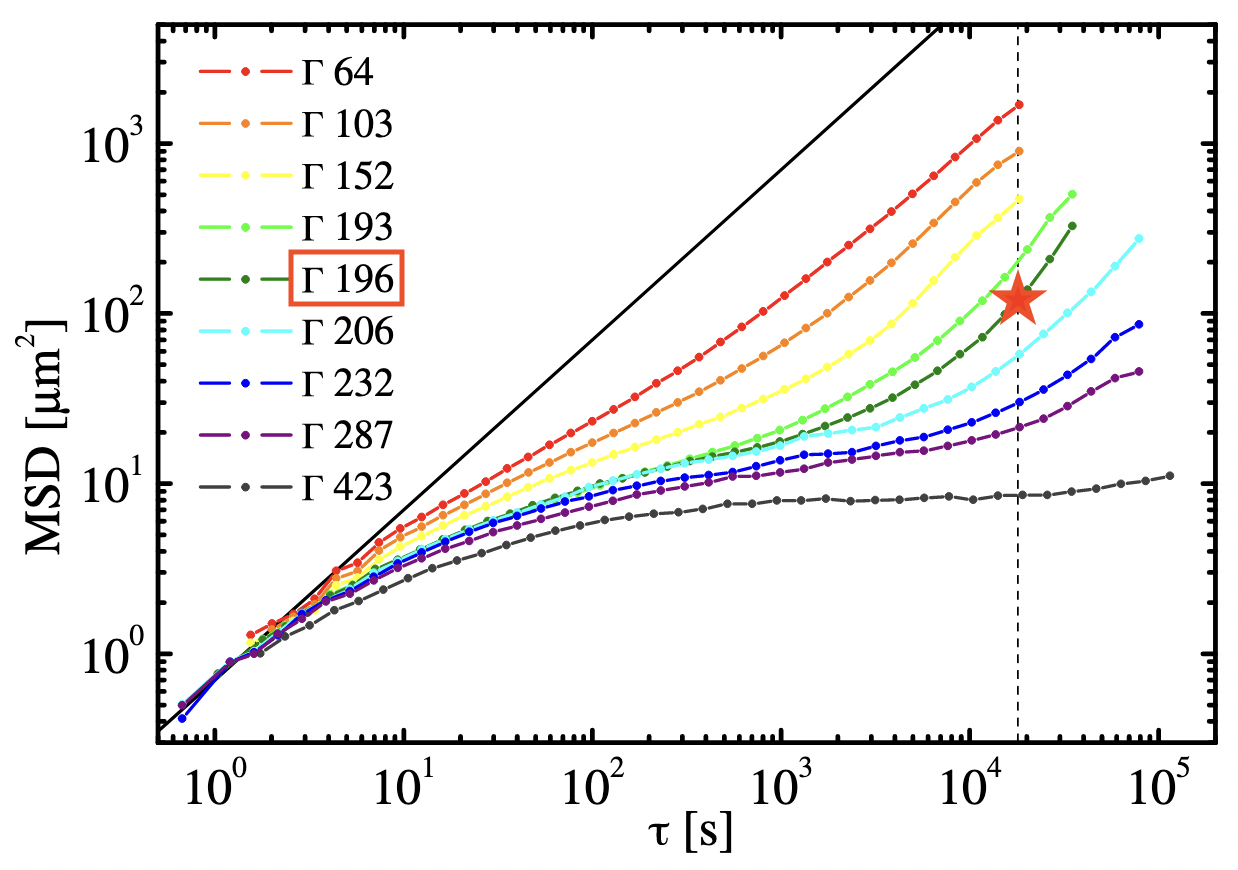
\includegraphics[width=0.9\linewidth]{9.d-kt_keim/msd_keim_1.png}\caption{Their MSD data indicates that the transition is occurring near the onset point for glassy dynamics  (Klix, Maret, and Keim \textit{Phys. Rev. X} 2015).}
%     \end{overprint}
%     \end{figure}
% \end{itemize}


% \end{column}

% \end{columns}  
% \end{frame}

\begin{frame}{A Theory of Onset Temperature in 2D: Young's Modulus as $T \to T_\mathrm{KT}$}

%\vspace{15pt}

\begin{columns}

\begin{column}[T]{0.425\textwidth}

\begin{figure}
    \begin{overprint}
    \onslide<4-5>\centering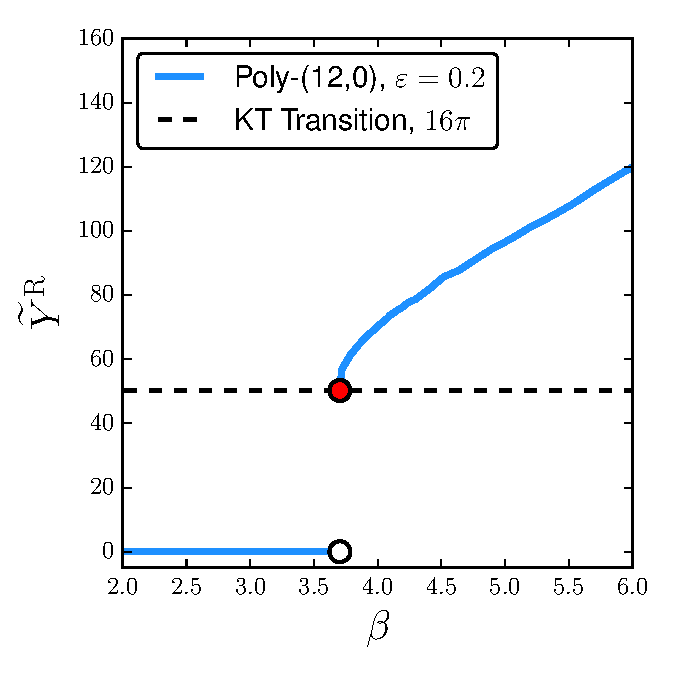
\includegraphics[height=0.65\textheight]{9.d-kt_keim/Yrenorm_poly12.pdf}\caption{The predicted Young's modulus according to RG calculations (discontinuity at $T=T_\mathrm{KT}$)}
    
    \onslide<6>\vspace{15pt}\centering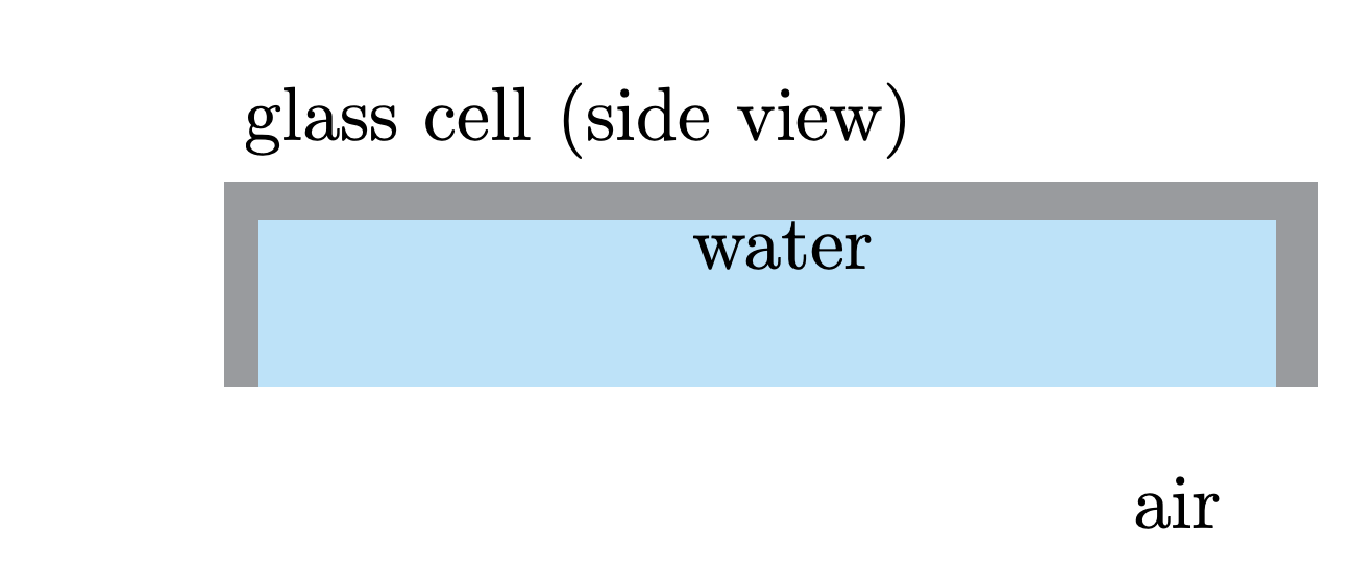
\includegraphics[width=\linewidth]{9.d-kt_keim/keim_setup_0.pdf}\caption{A colloidal system (polystyrene spheres) confined to a flat water-air interface (Ebert, et.al. \textit{Rev. Sci. Instrum} 2009).}
    
    \onslide<7>\vspace{15pt}\centering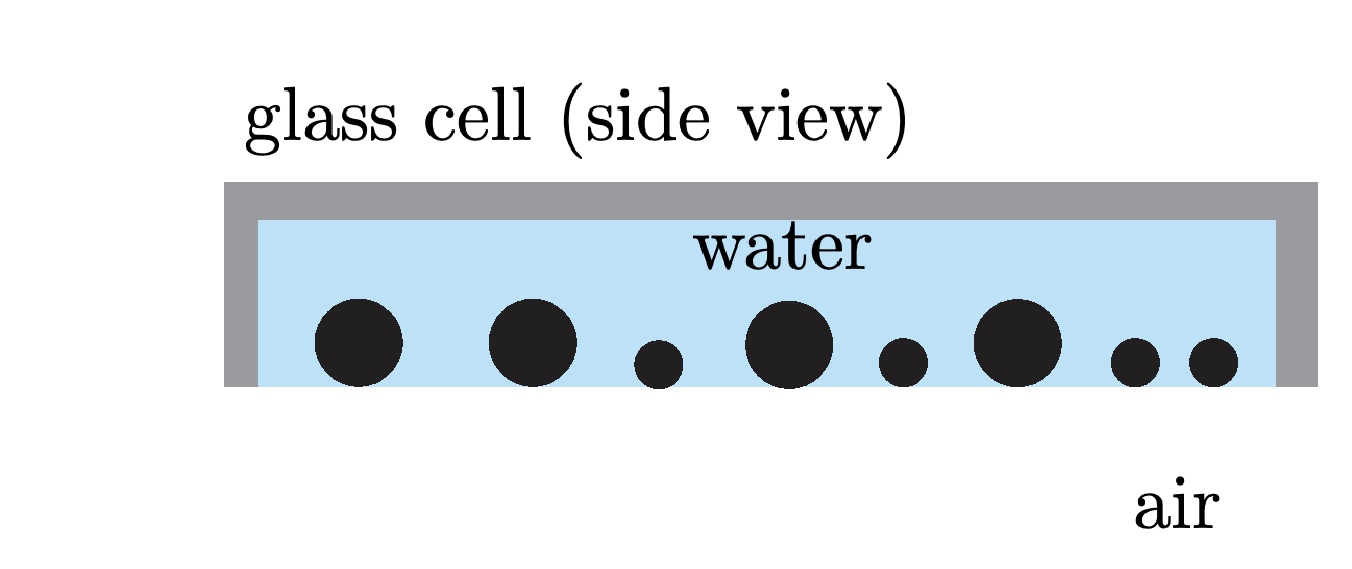
\includegraphics[width=\linewidth]{9.d-kt_keim/keim_setup_1.pdf}\caption{A colloidal system (polystyrene spheres) confined to a flat water-air interface (Ebert, et.al. \textit{Rev. Sci. Instrum} 2009).}
    
    \onslide<8>\vspace{15pt}\centering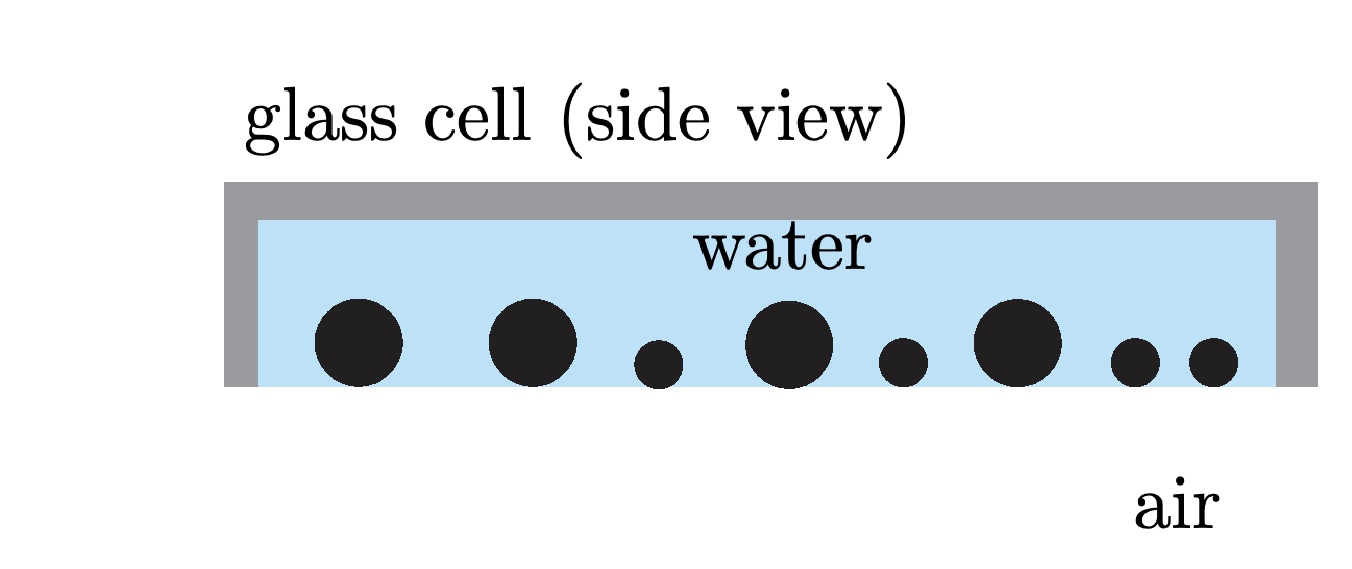
\includegraphics[width=\linewidth]{9.d-kt_keim/keim_setup_1.pdf}\caption{Each sphere is doped with magnetite}
    
    \onslide<9-10>\vspace{15pt}\centering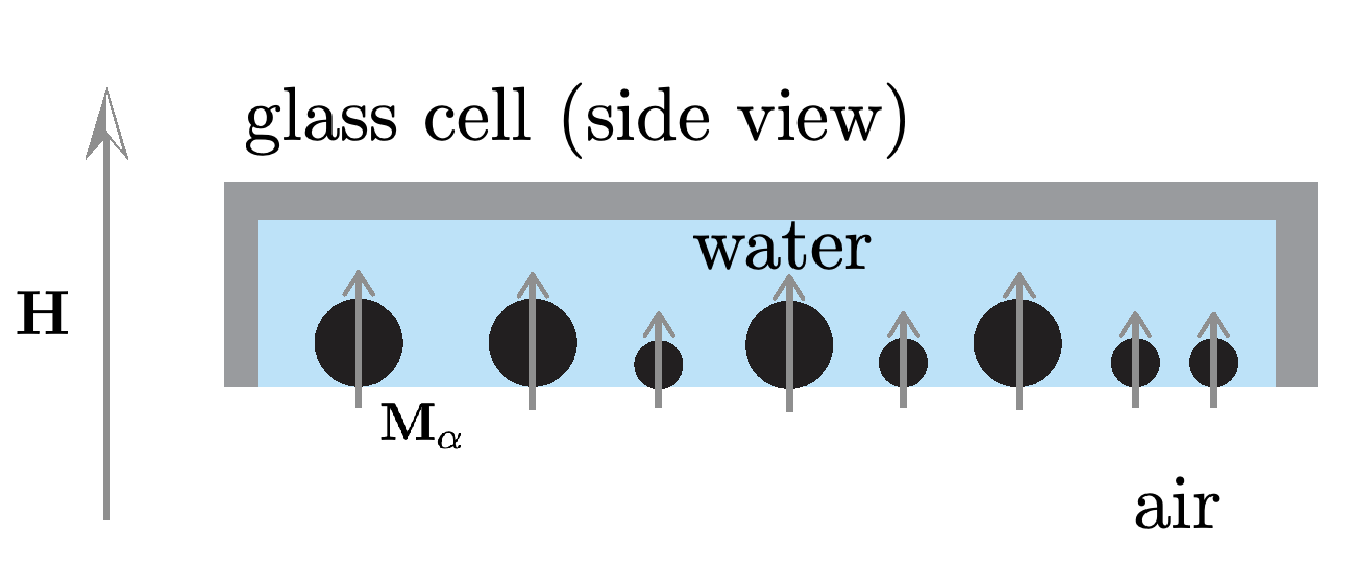
\includegraphics[width=\linewidth]{9.d-kt_keim/keim_setup_2.pdf}\caption{Each sphere is doped with magnetite $\to$ tuning of pair dipolar interaction between particles}
    
    \onslide<11>\centering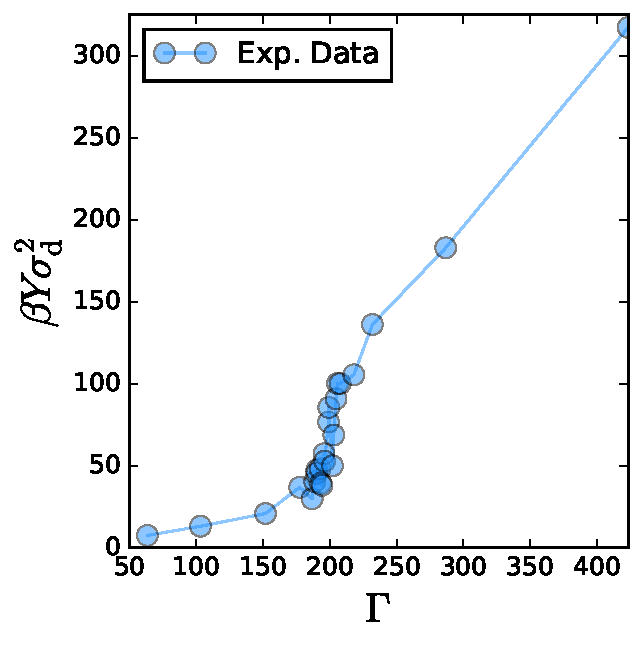
\includegraphics[height=0.65\textheight]{9.d-kt_keim/YRG_keim_exp_0.pdf}\caption{Young's modulus data, (re)computed from the bulk/shear moduli data.}
    
    \onslide<12>\raggedright\vspace{30pt}{\textit{Concerning the height of the jumps, we are not aware of predictions of universal behavior of elasticity in thermal amorphous systems as, e.g., \km{the famous $16 \pi \approx 50.26$ for Young's modulus in $2 \mathrm{D}$ melting} [40], but the measured values in glass and crystal are of} \textbf{the same order.} 
    \vspace{5pt}
    
    -- Klix, Maret, and Keim, \textit{PRX} 2015}
    

    \onslide<13>\centering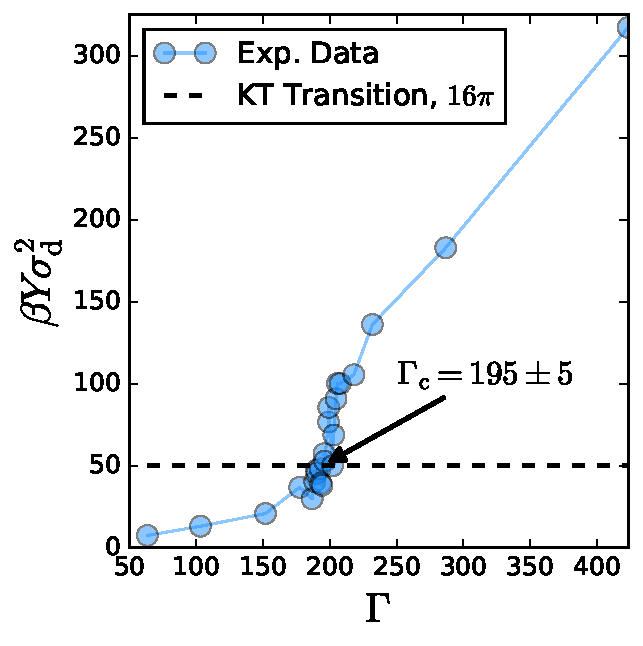
\includegraphics[height=0.65\textheight]{9.d-kt_keim/YRG_keim_exp_1.pdf}\caption{Young's modulus data, (re)computed from the bulk/shear moduli data.}
    
    \onslide<14>\centering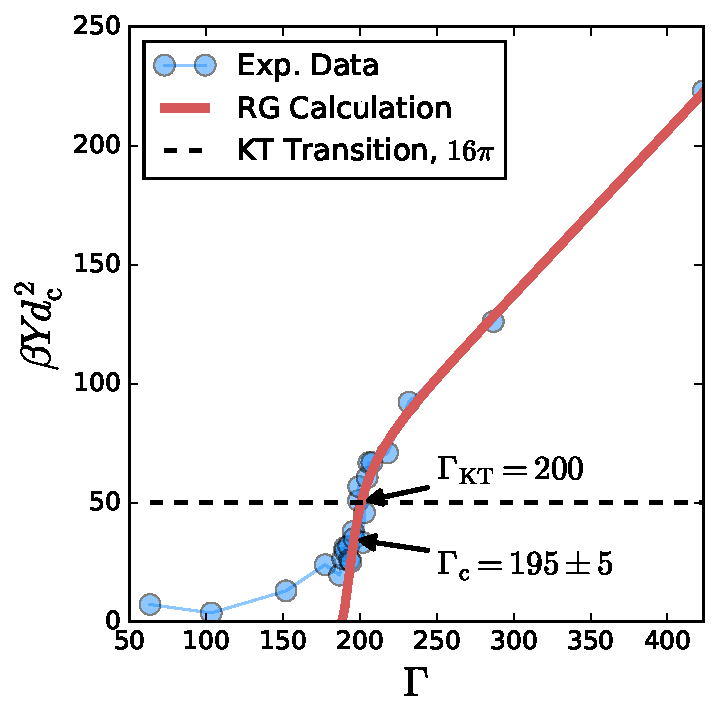
\includegraphics[height=0.65\textheight]{9.d-kt_keim/YRG_keim.pdf}\caption{Prediction agrees with experiments. Input: RDF and Young's modulus at high-$\Gamma$\vspace{-10pt}\footnote{ F. Ebert, Ph.D. Dissertation, 2008; C. Klix, Ph.D. Dissertation, 2014}.}
    
    \onslide<15>\centering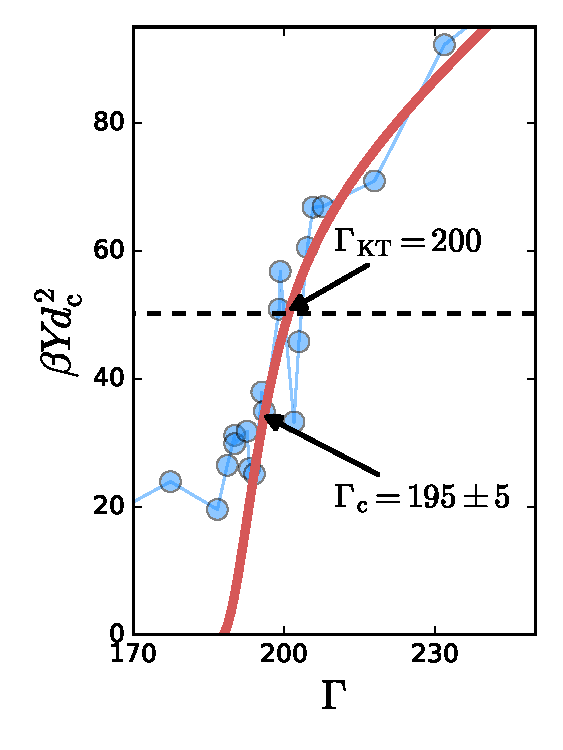
\includegraphics[height=0.75\textheight]{9.d-kt_keim/YRG_keim_closeup.pdf}\caption{A closeup of RG prediction with exp. data}
    
    \onslide<16>\vspace{20pt}\centering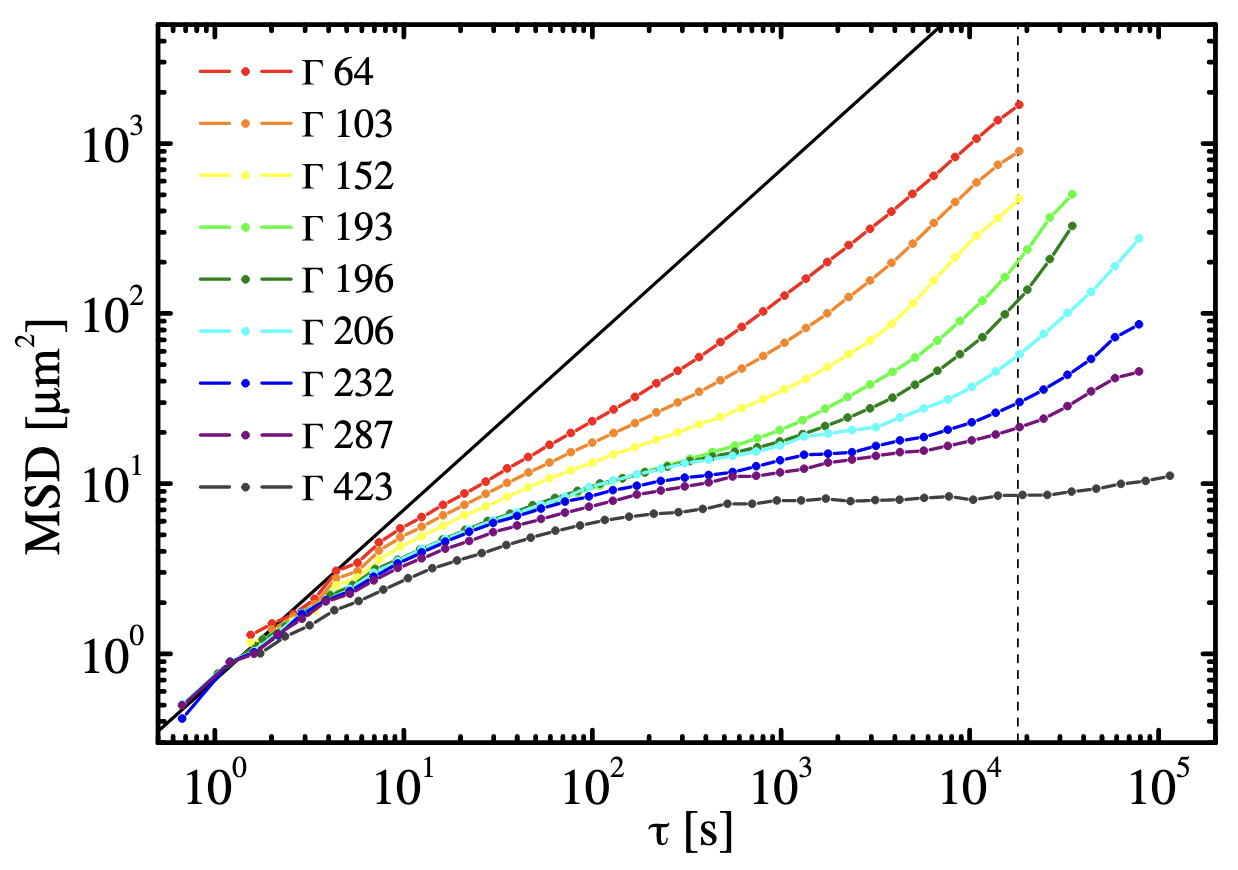
\includegraphics[width=\linewidth]{9.d-kt_keim/msd_keim.png}\caption{MSD data around the transition  (Klix, Maret, and Keim \textit{Phys. Rev. X} 2015).}
    
    \onslide<17>\vspace{20pt}\centering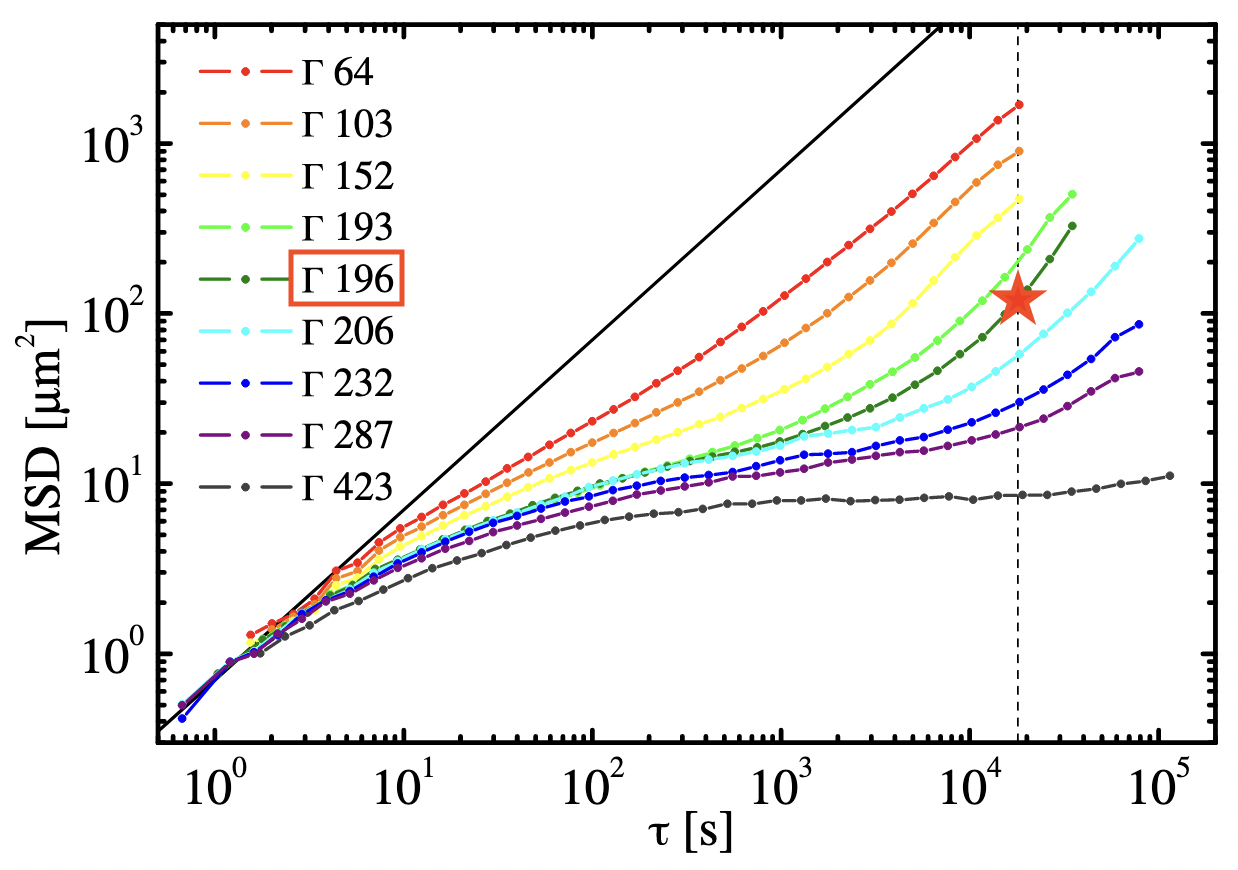
\includegraphics[width=\linewidth]{9.d-kt_keim/msd_keim_1.png}\caption{MSD data indicates that the transition is occurring near the onset point for glassy dynamics  (Klix, Maret, and Keim \textit{Phys. Rev. X} 2015).}
    
    % \onslide<19>\vspace{15pt}\centering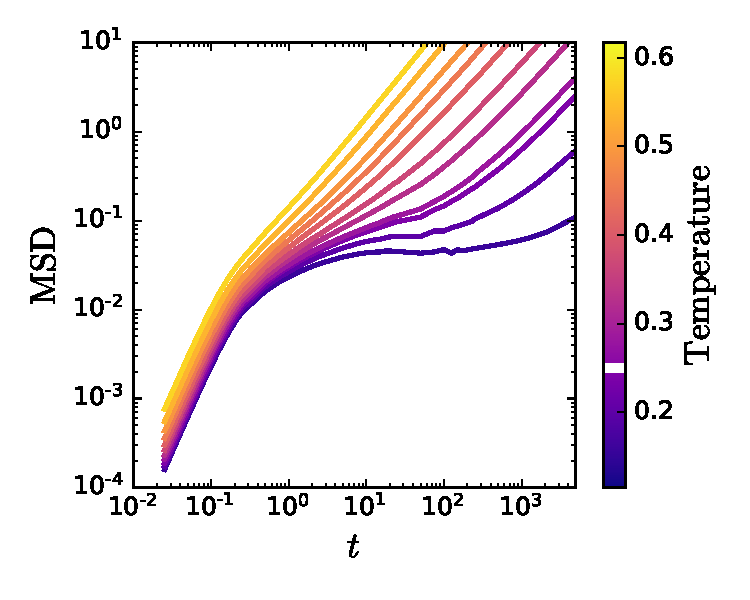
\includegraphics[width=\linewidth]{9.d-kt_keim/msd_poly12.pdf}\caption{MSD Data of Poly-(12,0) around $T_\mathrm{o}$ is qualitatively similar to experimental data.}
    
    \onslide<18->\centering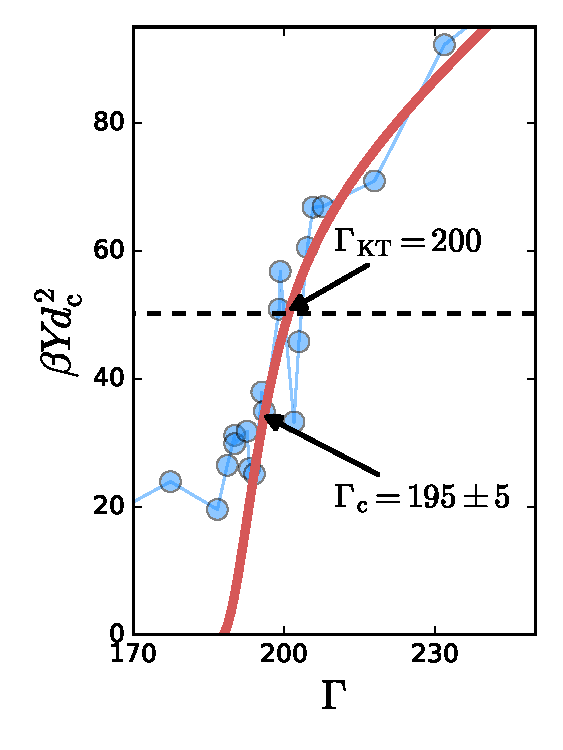
\includegraphics[height=0.75\textheight]{9.d-kt_keim/YRG_keim_closeup.pdf}%\caption{MSD Data of Poly-(12,0) around $T_\mathrm{o}$ is qualitatively similar to experimental data.}
    
    
    \end{overprint}
    \end{figure}
    

\end{column}

\begin{column}[T]{0.575\textwidth}


\begin{itemize}
    \item<2->Pick an intermediate time $\Delta t \ll \tau_\mathrm{eq}$ and measure strain fluctuations at $t = \Delta t$:
    \begin{equation*}
    \frac{1}{Y^\mathrm{R}} = \beta A_0 \left(\left\langle\hat{\epsilon}_{i j} \hat{\epsilon}_{i j}\right\rangle+\frac{1}{2}\left\langle\hat{\epsilon}_{i i}\hat{\epsilon}_{k k}\right\rangle\right)
    \end{equation*}
    \item<5-> Similar measurements have been done in an \textit{experimental} study (Klix, Maret, and Keim \textit{Phys. Rev. X} 2015)
    \onslide<10->{$${ \text{\textbf{Coupling strength}} \ \bm \Gamma} \sim \beta H^2 $$}
    \vspace{-18pt}
    \item<14-> Apply the RG theory given existing data available from Keim and Maret group.
    \onslide<18->\begin{block}{\centering Inherent-State Melting as a "Hidden" Transition}
    \vspace{5pt}
    \centering The mechanism is thermodynamic in character but observable dynamically at $t \ll \tau_\mathrm{eq}(T)$
    \vspace{5pt}
    \end{block}

\end{itemize}


\end{column}

\end{columns}  
\end{frame}